\documentclass[11pt, oneside]{article} 
\usepackage{geometry}
\geometry{letterpaper} 
\usepackage{graphicx}
	
\usepackage{amssymb}
\usepackage{amsmath}
\usepackage{parskip}
\usepackage{color}
\usepackage{hyperref}

\graphicspath{{/Users/telliott_admin/Tex/png/}}
% \begin{center} 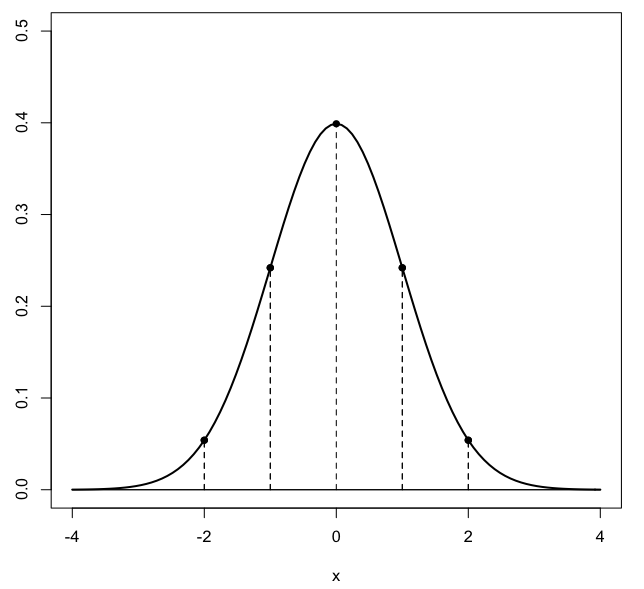
\includegraphics [scale=0.4] {gauss3.png} \end{center}

%break
\title{Polar coordinates}
\date{}

\begin{document}
\maketitle
\Large
In polar coordinates points are plotted in terms of distance from the origin, $r$ and the angle $\theta$ that this ray makes with the positive $x$-axis.  Converting from $x,y$ to $r, \theta$ is pretty easy:
\[ x = r \cos \theta \]
\[ y = r \sin \theta \]

To go the other way, use Pythagoras to write 
\[ x^2 + y^2 = r^2 \]
\[ \theta = \tan^{-1} (\frac{y}{x}), \ \ x \ne 0 \]

In polar coordinates, as in Cartesian ($xy$) coordinates, the equation of a circle depends on whether it is at the origin or not.  If it is at the origin, then something like
\[ r = 3 \]

defines the graph.  But if it's away from the origin, then the equations are of the form:
\[ r = a \cos \theta + b \sin \theta \]

Let's do a derivation and then look at examples.  We can manipulate these equations to go back to Cartesian coordinates.
\[ r = 2h \cos \theta + 2k \sin \theta \]

The reason for choosing these particular coefficients will become clear shortly.  Substitute  $x$ and $y$.
\[ r = 2h \cdot \frac{x}{r} + 2k \cdot \frac{y}{r} \]
so 
\[ r^2 = 2hx + 2ky \]
\[ x^2 + y^2 = 2hx + 2ky \]
\[ [ \ x^2 - 2hx  \ ] \ + \  [ \ y^2 - 2ky  \ ]  \ = 0 \]
complete both squares
\[ [ \ x^2 - 2hx + h^2 \ ] \ + \  [ \ y^2 - 2ky + k^2 \ ]  \ = h^2 + k^2 \]
\[ (x - h)^2 + (y - k)^2 = h^2 + k^2 \]

That is, for an equation of the form
\[ r = 2h \cos \theta + 2k \sin \theta \]

the origin is at $(h,k)$ and the radius is
\[ r = \sqrt{h^2 + k^2} \]

If the equation contains only $\sin \theta$ then compute $k$ equal to one-half the coefficient of $\sin \theta$, with the origin at $(0,k)$ and radius $r = k$.

Similarly, if the equation contains only $\cos \theta$ then compute $h$ equal to one-half the coefficient of $\cos \theta$, with the origin at $(h,0)$ and radius $r = h$.

\subsection*{examples}
For example
\[ r = 3 \sin \theta \]

is a circle centered at $(0,3/2)$, with a radius of $3/2$ (it passes through the origin and the point $(x=0,y=3)$.  All such circles (with just one of $\sin \theta$ or $\cos \theta$) have this property.

And
\[ r = \sin \theta + \cos \theta \]
is a circle centered at $(1/2, 1/2)$ with a radius squared:
\[ r^2 = h^2 + k^2 = (\frac{1}{2})^2 + (\frac{1}{2})^2 = \frac{1}{2} \]
\[ r = \frac{1}{\sqrt{2}} \]
We see that all circles of this form pass through the origin.

\begin{center} 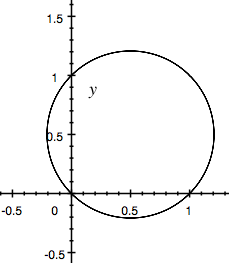
\includegraphics [scale=0.6] {polar_circle.png} \end{center}

\subsection*{other conic sections}
Parabolas look like this:

\[ r = \frac{1}{1 \pm a \sin \theta} \]
\[ r = \frac{1}{1 \pm a \cos \theta} \]

The ones with $\sin \theta$ open up and down, the others open left and right.  If the sign of the $a$ term is negative, the parabola opens up or to the right.

The general formulas are
\[ r = \frac{ep}{1 \pm e \sin \theta} = p \ \frac{1}{1/e + \sin \theta} \]
\[ r = \frac{ep}{1 \pm e \cos \theta} = p \ \frac{1}{1/e + \cos \theta} \]

where $e$ is the eccentricity ($e = 1$ for a parabola).  If $e < 1$ then we have an \textbf{ellipse}.

\subsection*{parabola}

Consider
\[ r = \frac{2}{1 + \sin \theta} \]

Plot it to see.  Or convert to Cartesian coordinates:
\[ r  + r \sin \theta = 2 \]
\[ \frac{y}{r} = \sin \theta \]
\[ r + y = 2 \]
\[ r^2 = (2-y)^2  = x^2 + y^2 \]
\[ 4 - 4y + y^2 = x^2 + y^2 \]
\[ y - 1 = -\frac{1}{4} x^2  \]

\subsection*{ellipse}
If we measure $r$ and $\theta$ from a focus, then
\[ x = c + r \cos \theta \]
\[ y = r \sin \theta \]

one can derive a formula for the ellipse in terms of $r,\theta$
\[ r = \frac{ep}{1 \pm e \cos \theta} \]
(We talk more about this \hyperref[sec:Polar_ellipse]{\textbf{here}}).  For example if
\[ r = \frac{1}{1 + e \cos \theta} \]
with $0 < e < 1$, we will get an ellipse.
\end{document}  